\mkexercise{Diseñar un Amplificador en configuración de emisor común
con un transistor tipo Q2N2222A (BIPOLAR.OLB) que tenga una ganancia
en tensión $A_v=10$ y una impedancia de entrada $Z_{in} = 250
\Omega$. El amplificador debe alimentarse a una batería de 12 $V$
sobre una carga de salida dependiente del $DNI: RL = 1000+(DNI \cdot
0.5) \Omega$ siendo $DNI$ las tres primeras cifras menos
significativas del documento. Los condensadores de paso y acoplo son
los indicados en el esquemático. La red de polarización debe ser
estable. La tensión térmica a $27^\circ$ es $V_T=25.85 mV$, la tensión
Early del transistor $V_{AF}=74.04 V$, la resistencia fenomenológica
del transitor es $RX=10\Omega$ y la $\beta_{DC}$ del transistor sigue
la siguiente dependencia con la corriente de colector:
}
  \begin{figure}[H]
    \centering  
    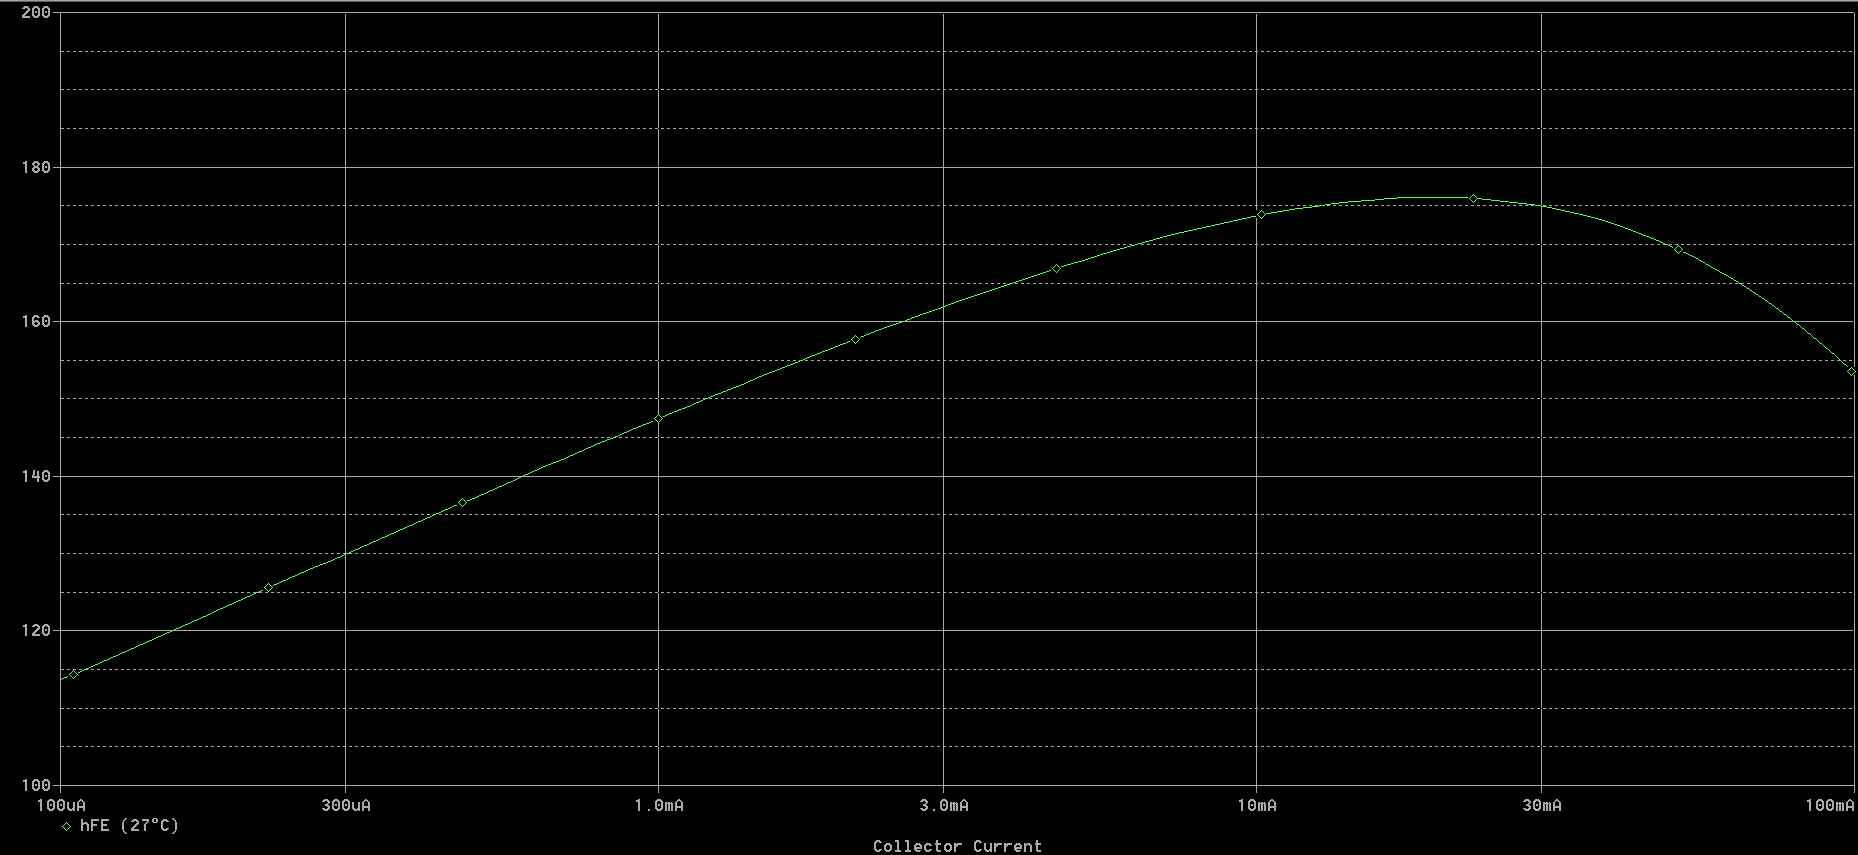
\includegraphics[scale=0.35]{images/beta.png}
    % izquierda,abajo,derecha,arriba
    \caption{Beta vs. $I_C$}
  \end{figure}

    \begin{figure}[H]
    \centering  
    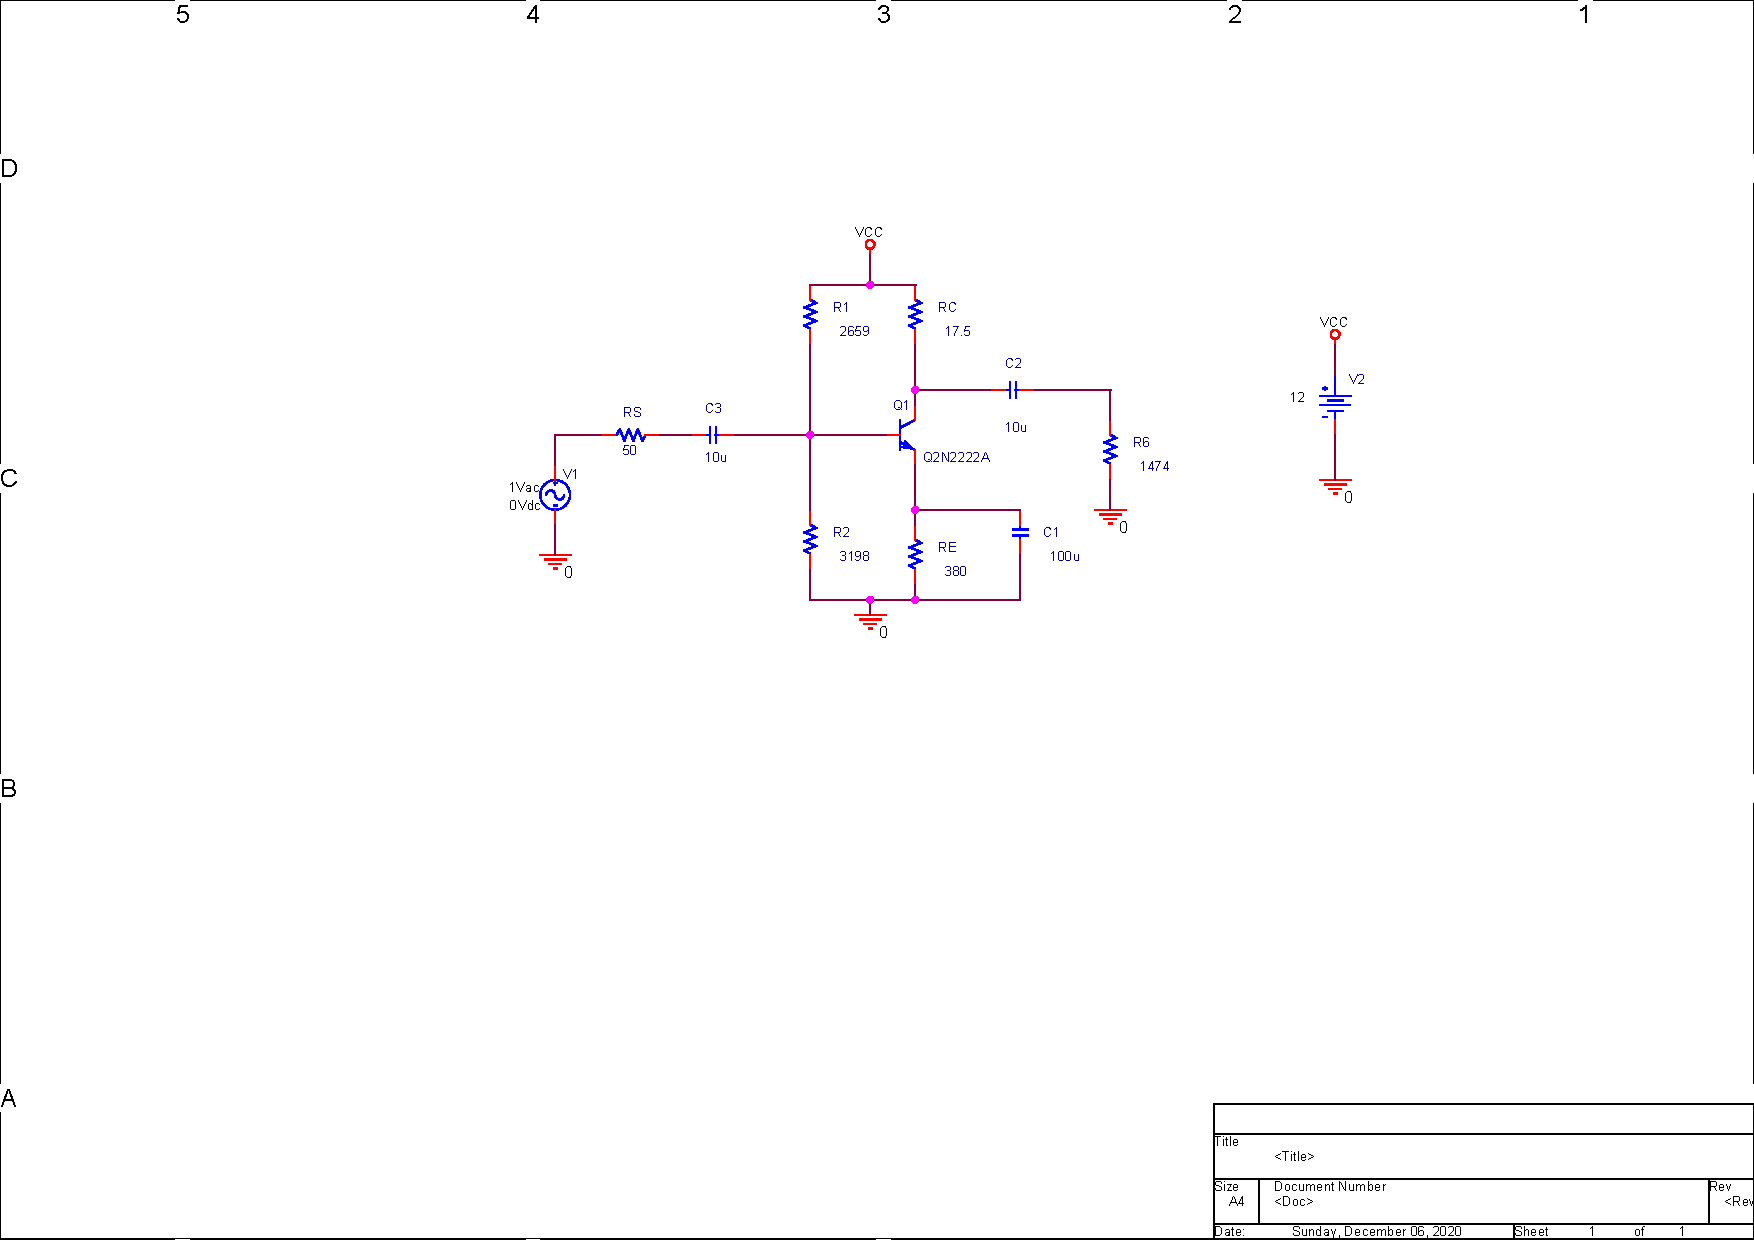
\includegraphics[scale=1,page=1,clip, trim=8cm 9.5cm 5cm 3.5cm]{images/problema_puntuable_5_sch.pdf}
    % izquierda,abajo,derecha,arriba
    \caption{Amplificador esquema}
  \end{figure}



Especificaciones de partida:
\begin{itemize}
\item $Z_{in}=250 \Omega$
\item $|A_V|=10$
\item $RL=1474$
\item $V_{cc}=12V$
\end{itemize}

    \begin{figure}[H]
    \centering  
    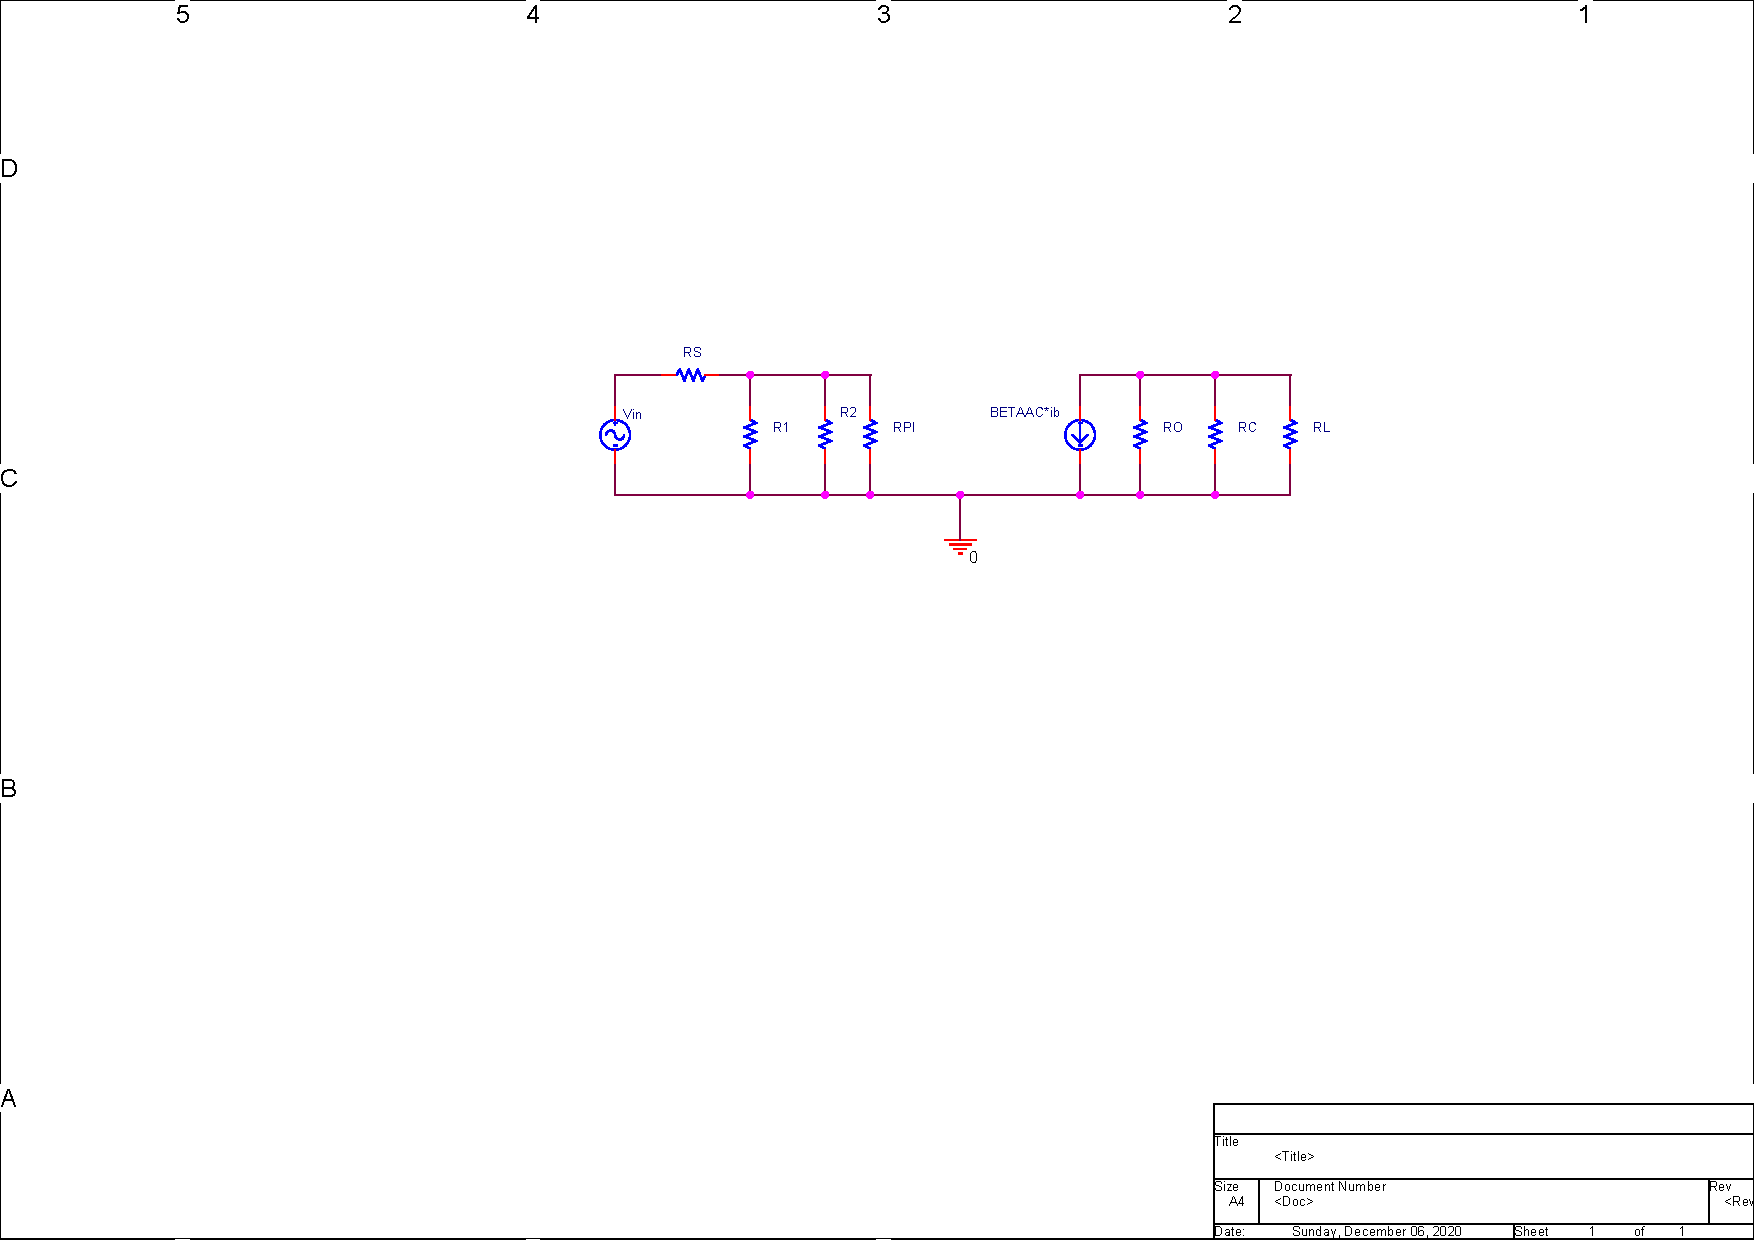
\includegraphics[scale=1,page=1,clip, trim=8cm 12cm 6cm 5cm]{images/modelo pi simplificado.pdf}
    % izquierda,abajo,derecha,arriba
    \caption{Amplificador esquema}
  \end{figure}
  
\begin{center}
\large\textbf{Parámetros del amplificador}
\end{center}

\begin{itemize}
\item \textbf{Impedancia de entrada}
  \[R_{in}=R_{\pi}||RB = 250 \Omega \]
  El paralelo de dos resistencias es menor que el menor valor de
  ellas, RPI > 250 $\Omega$ pero no debemos pasarnos porque si no RPI
  sería despreciable y $R_{in} \simeq RB$.
\item \textbf{Impedancia de salida}
\begin{center}
Parámetro no fijado
\end{center}
\item \textbf{Ganacia en corriente}
\begin{center}
Parámetro no fijado
\end{center}
\item \textbf{Ganancia en tension}
\[|A_{V}| = GM\cdot(RO||RC||RL) = 10\]
\end{itemize}

\begin{center}
  \large\textbf{Parámetros de pequeña señal}
\end{center}

\begin{itemize}
\item $R_{\pi}$
  \[R_{\pi} = \dfrac{\beta}{GM}\]
\item $GM$
  \[GM   = \dfrac{I_C}{V_T}\]
  \item $RO$
    \[RO= \dfrac{V_{CE}+V_{AF}}{I_C}\]
\end{itemize}

En este punto por el camino que hemos seguido debemos seleccionar una
$I_c$ y una $\beta$ pero dado que estoy siguiendo la solución del
problema puntuable 5 y que sé que que la estabilidad es aceptable
usaré directamente $I_C = 15 mA$ y  $\beta=175$ aunque lo normal
sería realizar una primera aproximación para identificar los
parámetros deseados del diseño final.

\begin{equation}
R_{\pi} = \dfrac{\beta \cdot V_T}{I_C}=\dfrac{175\cdot
\mili{25.85}\ V}{\mili{15} \ A} = 302 \Omega > 250 \Omega
\end{equation}

\begin{equation}
RB = \dfrac{Z_{in} \cdot P_{\pi}}{R_{\pi}-Z_{in}} = \dfrac{250 \cdot
302}{302-250} = 1452 \Omega 
\end{equation}

\begin{equation}
  GM = \dfrac{I_c}{V_T} = \dfrac{\mili{15}\ A}{\mili{25.85}\ V} =
  0.580 \ A/V
\end{equation}

\begin{equation}
RO = \dfrac{V_{CE}+V_{AF}}{I_C} = \dfrac{6+74.04}{\mili{15}} = 5336 \Omega
\end{equation}

\begin{equation}
RC = \dfrac{\dfrac{|A_V|}{GM}\left(RO||RL\right)}{\left(RO||RL\right)-\dfrac{A_V}{GM}}
= \dfrac{\dfrac{10}{0.580}(1155)}{(1155)-\dfrac{10}{0.580}} = 17.50 \Omega
\end{equation}

\begin{equation}
RE = \dfrac{V_{cc}-V_{CE}-RC\cdot I_C}{\dfrac{\beta+1}{\beta} I_C} =
\dfrac{12-6-17.50\cdot \mili{15}}{\dfrac{175+1}{175}\mili{15}} = 380
\Omega 
\end{equation}

Si calculamos el factor de inestabilidad, obtenemos:
\begin{equation}
S_{I_{CO}}^{I_C}= 1 + \dfrac{RB}{RE} = 1 + \dfrac{1452}{380} = 4.82 
\end{equation}

Valor cercano a la cota inferior de estabilidad de la red  de
polarización.

Calcularemos $R_1$ y $R_2$ mediante la tensión Thevening en el nodo
$V_B$:
\begin{equation}
  \begin{split}
    V_B & = \dfrac{V_{cc}\cdot R_2}{R_1+R_2}\\
    V_B & = RB \cdot I_B + V_{BE} + RE(I_B+I_C)\\
    I_B & = \dfrac{I_C}{\beta} = \dfrac{\mili{15}}{175} = 85.71\mu A\\
    V_B & = 1452 \cdot \micro{85.71} +0.7 + 380 (\mili{85.71}+\mili{15})\\
    V_B & = 6.55 \ V \\
    \dfrac{V_B}{V_{cc}} & = \dfrac{R_2}{R_1+R_2} = \dfrac{6.55}{12} \\
    \dfrac{V_B}{V_{cc}} & = 0.546 \\
    R_1 & = \dfrac{1452}{0.546} = 2659 \Omega\\
    R_2 & = \dfrac{1452}{1-0.546} = 3198 \Omega\\
    \end{split}
  \end{equation}

Resumen de las resistencias de polarización:
\begin{itemize}
\item RC = 17.5 $\Omega$
\item RE = 380 $\Omega$
\item $R_1$ = 2659 $\Omega$
\item $R_2$ = 3198 $\Omega$
\end{itemize}

Llevamos el circuito al simulador y obtenemos los siguientes
resultados:

    \begin{figure}[H]
    \centering  
    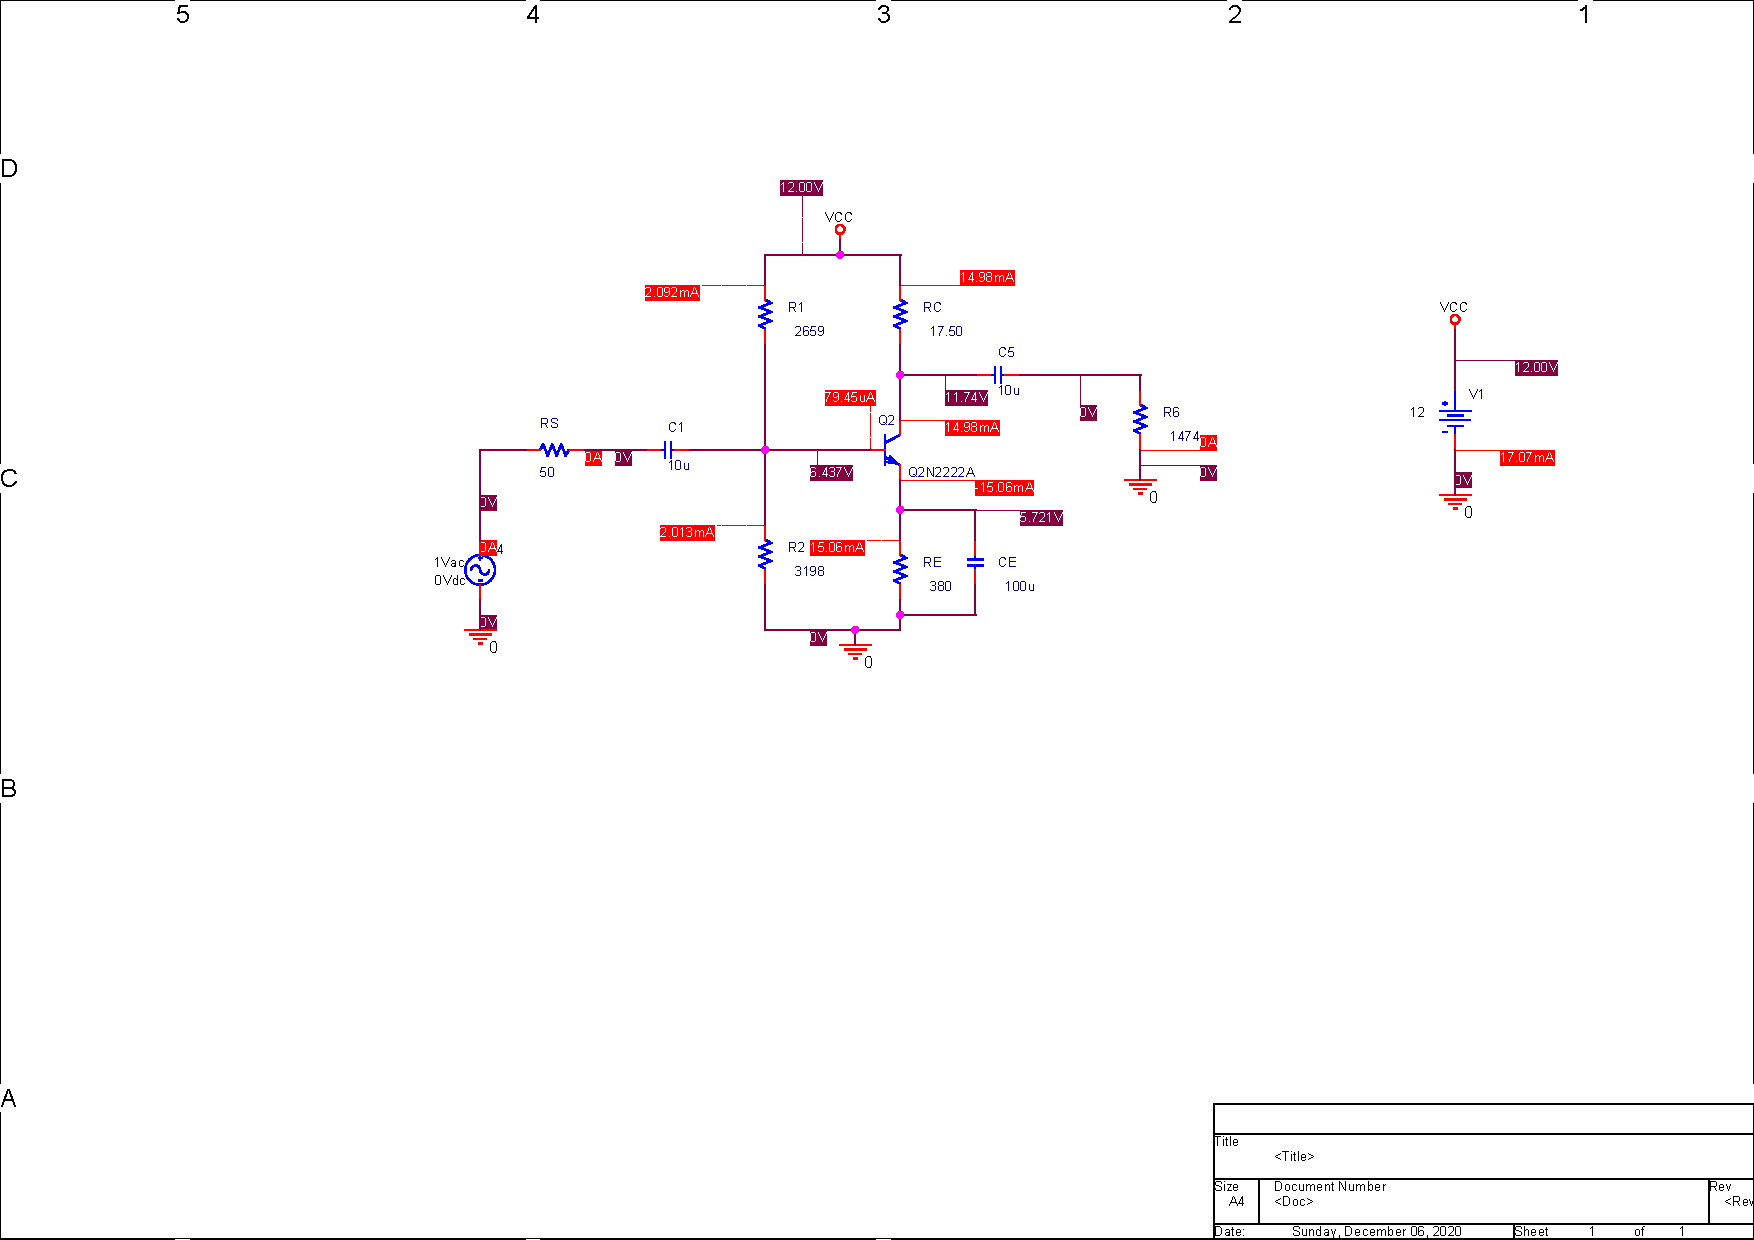
\includegraphics[scale=0.8,page=1,clip, trim=7.5cm 9cm 2cm
    2cm]{images/biaspoint_problema_puntuable.pdf}
    % izquierda,abajo,derecha,arriba
    \caption{Bias point}
  \end{figure}
      \begin{figure}[H]
    \centering  
    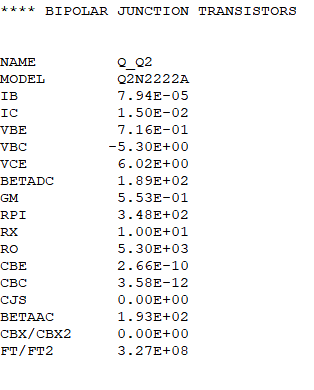
\includegraphics[scale=1]{images/model.png}
    % izquierda,abajo,derecha,arriba
    \caption{Output file - Model}
  \end{figure}

Si cogemos los datos del ``output file'' podemos calcular la
impedancia real de entrada y/o dispersión.

\[Z_{in} = R_{\pi}||RB = 348||1452 = 281\]
Esto da una dispersión del $11\%$ y una ganancia en tensión de:

\[|A_V| = GM \cdot (RO||RC||RL) = 0.553 \cdot (5336||17.5||1474) =
  9.53 \]
con una dispersión del $4.7\%$.

Los resultados son casi exactos a nivel analítico principalmente por
la carga ya que la variación que puede incluir la carga RL será
probablemente en los decimales que hemos eliminado con el redondeo.
\begin{figure}[H]
    \centering  
    \includegraphics[scale=0.45,page=2,trim]{images/problema_puntuable_5.pdf}
    % izquierda,abajo,derecha,arriba
    \caption{Ganancia en tensión}
  \end{figure}

  \begin{figure}[H]
    \centering  
        \includegraphics[scale=0.45,page=3,trim]{images/problema_puntuable_5.pdf}
    % izquierda,abajo,derecha,arriba
    \caption{Fase ganancia en tensión}
  \end{figure}

% ganancia en tensión
Se observa la ganancia constante a frecuencias intermedias de 9.2635,
difiere de la especificación de partida en 0.7365 considerando que el
simulador usa el modelo completo es una aproximación buena.

También podemos calcular los otros valores como $Z_{out},Z_{in},I_V$
    \begin{figure}[H]
    \centering  
    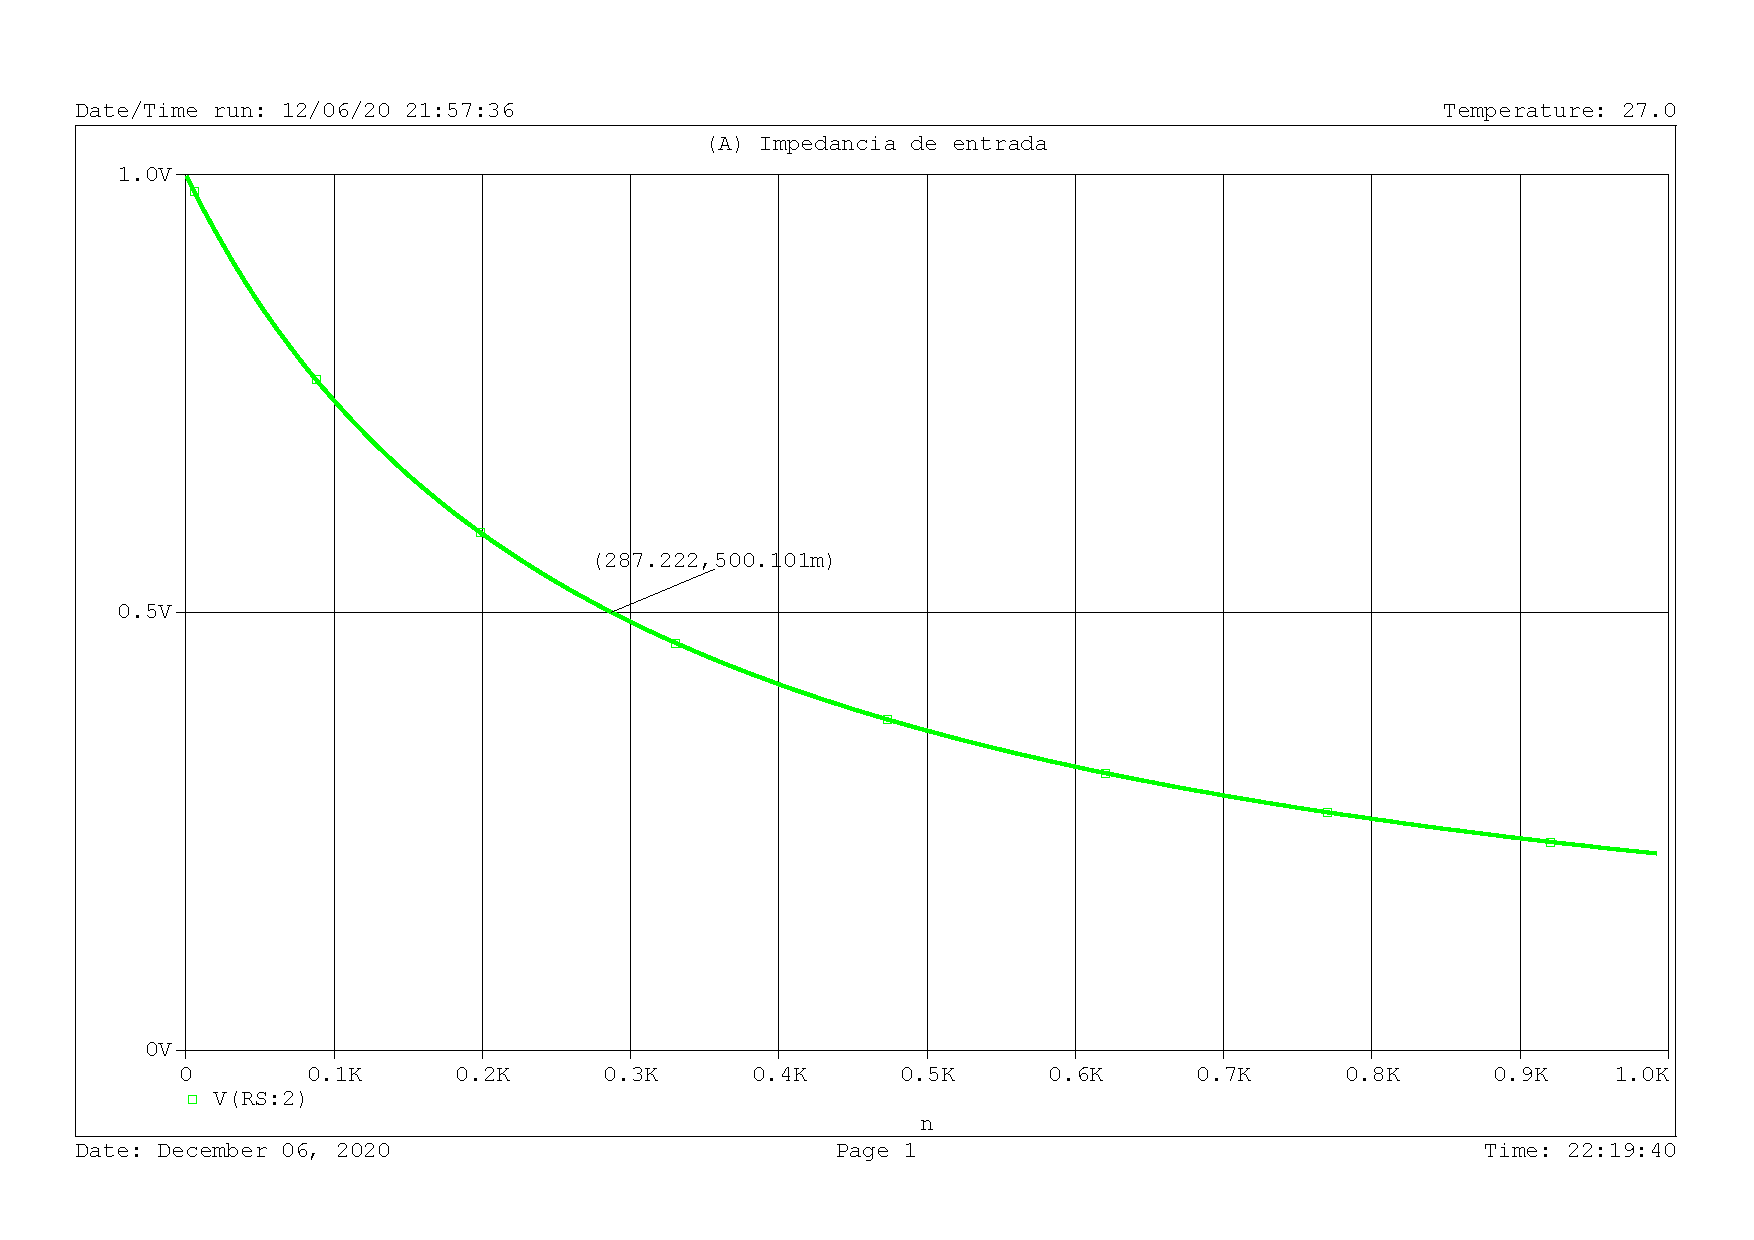
\includegraphics[scale=0.45,page=1,trim]{images/problema_puntuable_5.pdf}
    % izquierda,abajo,derecha,arriba
    \caption{Impedancia de entrada}
  \end{figure}
  Esta impedancia era esperada ya que con los valores del ``output
  file'' hemos podido calcular el $Z_{in}$ y su correspondiente
  dispersión en apartados anteriores.
  
    \begin{figure}[H]
    \centering  
    \includegraphics[scale=0.45,page=4,trim]{images/problema_puntuable_5.pdf}
    % izquierda,abajo,derecha,arriba
    \caption{Ganancia en corriente}
  \end{figure}
  Aunque la ganancia en corriente no era el objetivo de este
  amplificador es interesante observar el valor que puede proporcionar
  este topología.
      \begin{figure}[H]
    \centering  
    \includegraphics[scale=0.42,page=5,trim]{images/problema_puntuable_5.pdf}
    % izquierda,abajo,derecha,arriba
    \caption{Fase ganancia en corriente}
  \end{figure}

  Se puede ver el pequeño rango de frecuencias (siempre intermedias)
  en el que la señal no ``sufre'' un desfase durante la amplificación.
      \begin{figure}[H]
    \centering  
    \includegraphics[scale=0.42,page=6,trim]{images/problema_puntuable_5.pdf}
    % izquierda,abajo,derecha,arriba
    \caption{Impedancia de salida}
  \end{figure}

  La impedancia de salida es muy próxima a la calculada de forma analítica.\\

  
\begin{center}
  \textbf{Notas}
\end{center}

Como se puede ver hemos obtenido los mismos resultados, al no salir
mucho de los valores escogidos en la solución analítica es normal.

% Adjunto mis notas hechas

Antes de seguir el guión he intentado hacer un desarrollo propio, he
seguido dos caminos el primero modificar valores de $B_{AC}$ e $I_C$ y
el segundo hacer un desarrollo matemático extenso considerando el
modelo del transistor $R_{\pi}$ con la $R_x$, en ambos casos he tenido
problemas, el diseño en general no es algo fácil sin experiencia.

\begin{itemize}
\item Primer caso: Modificaciones en $B_{AC}$ - $I_C$.
  El cuello de botella principal en este intento era la gráfica del
  PSPICE MODEL EDITOR no hay cursores y es complicado usar la función
  $f(I_C) = \beta$, es uno de los motivos por los que seguí los
  resultados de la solución en el campus.

  Aunque este intento haya sido un fracaso total se puede observar
  perfectamente la influencia de la corriente del colector ya que una
  ligera modificación de $-5 mA$ ha generado una $RO = 8004 \Omega$
  que comparada con los resultados anteriores hay una diferencia de
  $3000 \Omega$ que no es muy poco, ni hablar de la $RC,RE,RB$ e
  incluso la estabilidad que seguía siendo menor de lo necesario.


\item Segundo caso: Desarrollo matemático.
  En este intento mi motivación era eliminar la complejidad de usar
  ecuaciones y reemplazar valores unos dentro de otros, además de
  fijar valores de modelado, como una estabilidad de 6, e incluso el
  uso del modelo en $\pi$ con una resistencia fenomenológica $R_X$. He
  obtenido $RB$s de 1900 $\Omega$ lo que da resistencias $R_1$ y $R_2$
  demasiado grandes de $3k\Omega$ y $4k\Omega$ aprox.
\end{itemize}

  Al final de esta pequeña sección adjunto parte de los intentos
  hechos por una simple prueba de lo interesante y complicado que puede ser el
  diseño en electrónica.

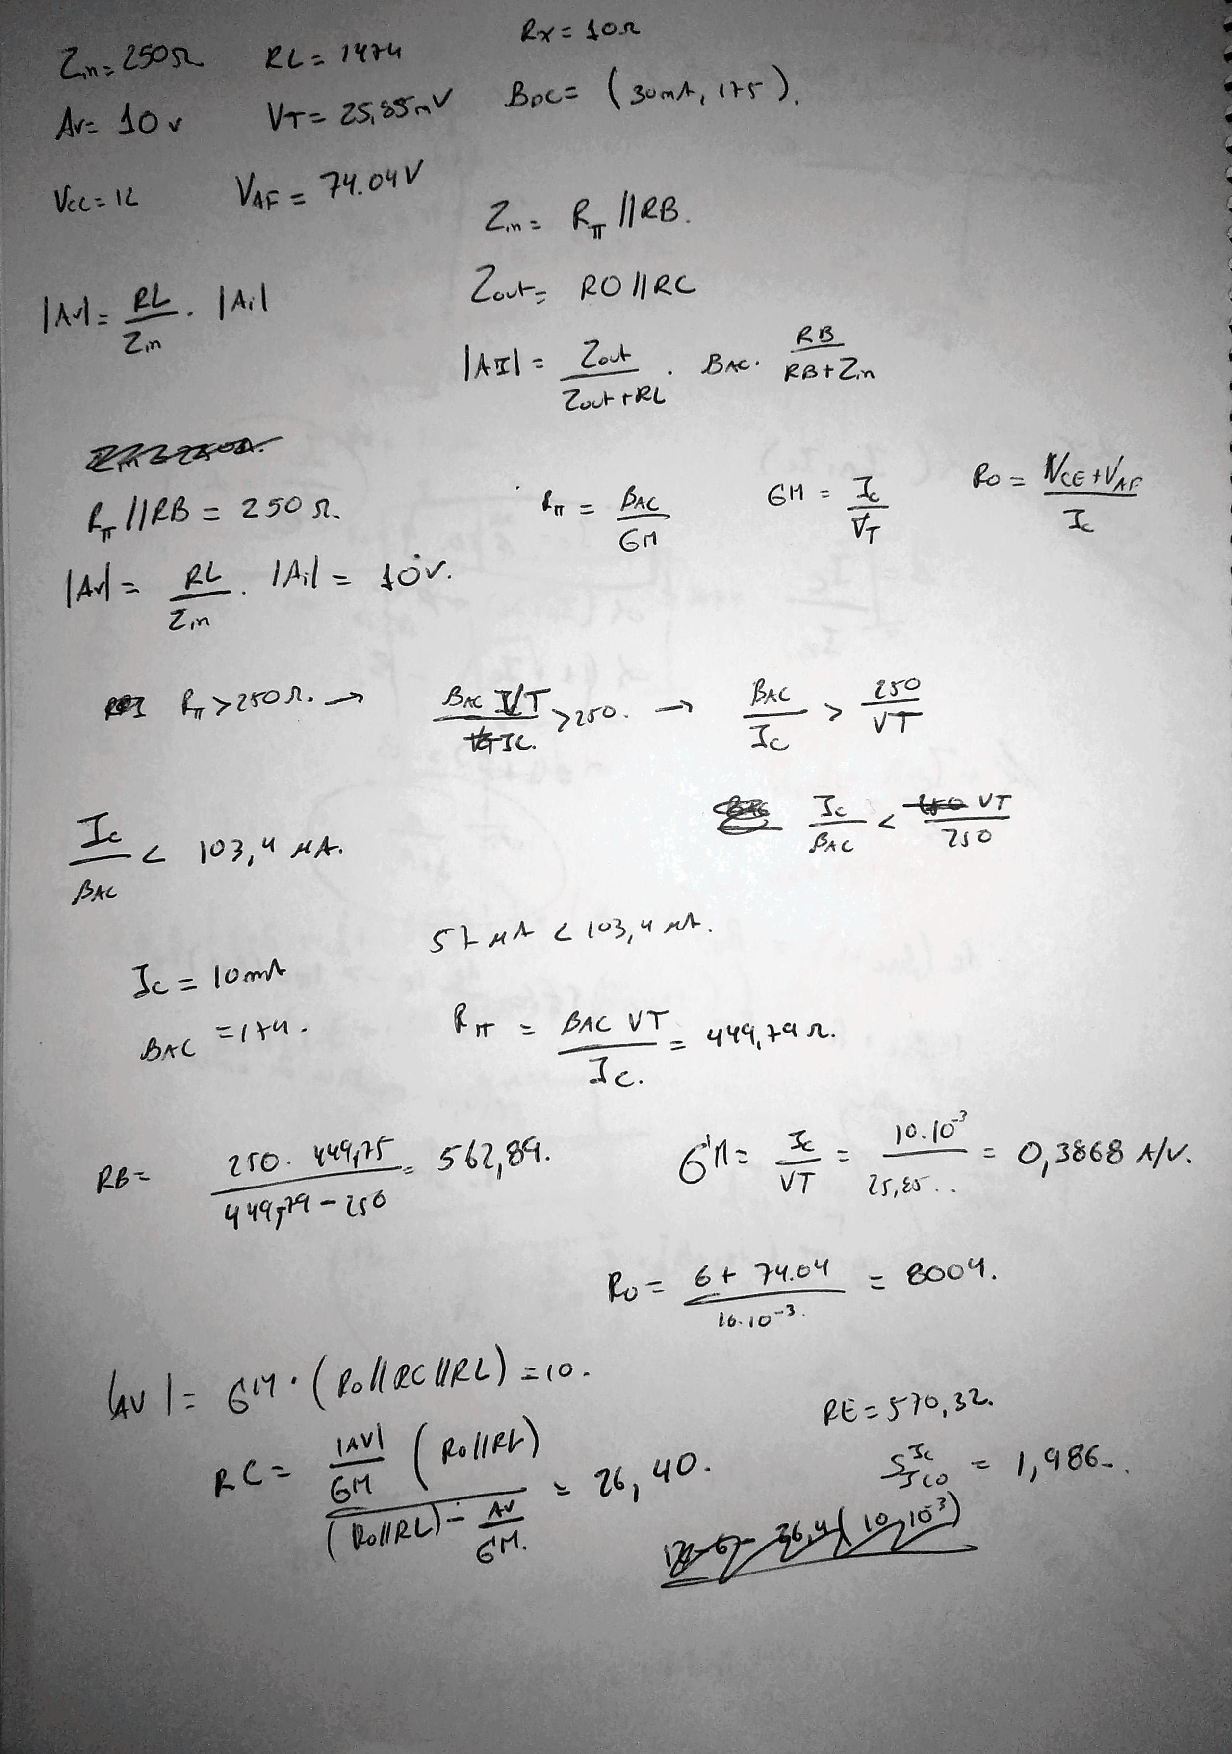
\includepdf[pages=-]{images/problema_puntuable_5_ana.pdf}